

\documentclass[aps,prd,twocolumn,superscriptaddress,nofootinbib]{revtex4-2}

\usepackage{graphicx}
\usepackage{amsmath}
\usepackage{amssymb}
\usepackage{wasysym}
\usepackage{hyperref}

\begin{document}

\title{Reconstructed-energy background spectra for a Quantum-Parity-Detector germanium wafer: reactor CEvNS, cosmic muons, and environmental gammas}

\author{Lanqing Yuan}
\email{yuan.l@wustl.edu}\affiliation{Washington University in St. Louis, St. Louis, Missouri, USA [PLACEHOLDER --- confirm affiliation and co-authors]}
\date{\today}

\begin{abstract}
Coherent elastic neutrino-nucleus scattering (CEvNS) from a nuclear reactor produces germanium nuclear recoils of only tens to hundreds of eV, at the threshold of emerging quantum sensors. We present an end-to-end forward model of the reconstructed-energy differential rate spectra measured by a thin ($4~{\rm in.}\times4~{\rm in.}\times2$~mm, $\sim$110~g) single-sided germanium wafer read out by Quantum Parity Detectors (QPDs), for two quasiparticle-trapping designs (Ta$\to$Al and Al$\to$Hf). On a single unified phonon energy scale with no ionization quenching, we compute the deposited-energy spectra of the reactor-CEvNS signal and of its surface backgrounds---sea-level cosmic muons, the environmental-gamma Compton continuum, the ambient fast-neutron elastic-recoil field, and the Ge-intrinsic cosmogenic decays of $^{3}$H, $^{68}$Ge, and $^{65}$Zn---and fold them through a Monte-Carlo QPD response matrix $R(E_{\rm rec}\,|\,E_{\rm dep})$ that includes the bandwidth-limited (25~kHz) censoring of the tunneling readout. The reconstructed energy is calibrated to estimate the deposited energy, so it doubles as the physical energy an experiment would report. Every rate is anchored to a published value or evaluated data library: the CEvNS rate reproduces the Billard \emph{et al.}\ (2017) germanium benchmark to within $2.4\%$, the integral muon rate matches the PDG sea-level flux within $\sim$$30\%$, the Compton edges fall at the Klein-Nishina energies, the neutron flux is normalized to the Gordon sea-level measurement, and the cosmogenic activities to SuperCDMS and EDELWEISS germanium measurements. The resulting spectra show that the reactor-CEvNS signal reconstructs to tens of eV---but it does not occupy that band alone: the ambient neutron-elastic recoils share its kinematics and, even after an assumed shield of NUCLEUS-demonstrated performance, are the dominant background in the $10$--$100$~eV region of interest, giving an in-band signal-to-background ratio of order a few ($S/B\simeq2.6$); the Ge-intrinsic cosmogenic decays, which no external shield reaches, set the irreducible floor beneath it. Cosmic-muon deposits saturate the readout and pile up into a tens-of-keV feature---an instrumental artifact of the bandwidth ceiling, not a physical spectral line---well clear of the signal band. We treat the saturated-regime response, the order-of-magnitude ambient-neutron rate and its assumed suppression, the site-dependent environmental-gamma normalization, and the sub-1.8~MeV reactor flux as explicit, quantified modeling uncertainties. This forward model maps the reconstructed-energy regime in which a QPD reactor-CEvNS search must operate, and carries the neutron-limited character of reactor-CEvNS backgrounds---already established in the field---through to a bandwidth-limited QPD readout.
\end{abstract}

\maketitle

\section{Introduction}
\label{sec:intro}
Coherent elastic neutrino-nucleus scattering (CEvNS) offers a compact, Standard-Model-anchored probe of reactor antineutrinos, but the nuclear recoils it produces in germanium at reactor energies are only tens to hundreds of eV, below the reach of conventional ionization or phonon detectors. First predicted by Freedman~\cite{freedman1974} and proposed as a neutrino-detection channel by Drukier and Stodolsky~\cite{drukier1984}, CEvNS was observed only in 2017 by the COHERENT experiment at a stopped-pion source~\cite{akimov2017}, which fixed the cross-section normalization against the electroweak Standard Model. Reactor sources move the target recoil energies an order of magnitude lower, into the tens-of-eV regime, in exchange for an enormous $\bar\nu_e$ flux. A dedicated effort has followed---CONUS+~\cite{conus2025}, Dresden-II~\cite{dresden2022}, and NUCLEUS~\cite{nucleus}---each pushing the deposited-energy threshold toward and below $100$~eV, where the germanium reactor-CEvNS rate is benchmarked by the calculation of Billard~\emph{et~al.}~\cite{billard2017}. The central experimental obstacle is not statistics but threshold: recovering the reactor-CEvNS spectrum demands sensitivity to nuclear recoils that terminate at a few tens of eV.

Quantum Parity Detectors (QPDs) are a superconducting readout concept aimed squarely at this regime~\cite{ramanathan2026}. A QPD infers a deposited energy from the population of quasiparticles it liberates in a superconducting sensor, sensed through the parity-dependent tunneling of individual quasiparticles across a Josephson junction. Because each tunneling event is counted, the scheme offers a path to sub-keV and even eV-scale thresholds on a fieldless phonon calorimeter. It carries, however, an intrinsic limitation: the tunneling signal is bandwidth-limited, and the readout response \emph{saturates} once the instantaneous tunneling rate exceeds the resolving ceiling---here $\sim$$25$~kHz, set by a $\tau_d\simeq40$~$\mu$s dead time. A large deposit drives the burst rate far above this ceiling, so the number of \emph{recorded} tunneling events, and hence the inferred energy, no longer tracks the energy actually deposited. The decisive observable for such a detector is therefore not the deposited energy but the \emph{reconstructed} energy $E_{\rm rec}$ that survives the bandwidth-limited counting chain. A background that is innocuous in deposited energy can, after reconstruction, land squarely on top of an eV-scale signal.

This paper computes that reconstructed-energy observable end to end. We build a forward model that maps the deposited-energy spectrum of the reactor-CEvNS signal and of its surface backgrounds into reconstructed-energy differential rate spectra $dR/dE_{\rm rec}$ for a thin single-sided germanium wafer read out by QPDs. The backgrounds are of three kinds: external electron-recoil continua from through-going cosmic-ray muons and the radiogenic environmental-gamma field; the external nuclear-recoil field of ambient fast neutrons, which scatter elastically off germanium and mimic the CEvNS signature directly; and the internal Ge-intrinsic decays of the cosmogenically activated isotopes $^{3}$H, $^{68}$Ge, and $^{65}$Zn, which deposit from inside the crystal and which no external shield can reach. We treat two quasiparticle-trapping designs, Ta$\to$Al and Al$\to$Hf~\cite{ramanathan2026}, and we place every channel on a single unified phonon energy scale with no ionization quenching, as befits a fieldless calorimeter, so that signal and backgrounds are directly co-added and folded through a common response. Every rate is anchored to a published value or evaluated data library rather than assumed: the deposited CEvNS rate reproduces the Billard germanium benchmark to within $2.4\%$, the cosmic-muon flux matches the sea-level value tabulated by the Particle Data Group to within its $\sim$$30\%$ inter-experiment spread~\cite{pdg}, the environmental-gamma Compton edges are fixed exactly by scattering kinematics, the ambient neutron flux is anchored to the Gordon sea-level measurement~\cite{gordon2004}, and the cosmogenic production rates to the SuperCDMS and EDELWEISS germanium-activation measurements~\cite{amman2019,edelweiss2017}. Because the external channels can be attenuated but the internal floor cannot, we present the background budget in an assumed-shield scenario---external muon, gamma, and neutron fields suppressed at the performance level demonstrated by NUCLEUS~\cite{nucleus}, the Ge-intrinsic floor carried unsuppressed. The response chain that carries these deposited spectra into $E_{\rm rec}$---the sensor-sharing partition, the tunneling-burst statistics, and the non-paralyzable censoring at the $25$~kHz ceiling---is the methodological core of the work.

The headline finding is a qualitative separation on the reconstructed axis. Because the reconstructed energy is calibrated to \emph{estimate} the deposited energy, the reactor-CEvNS signal, whose recoils lie entirely below the saturation onset, reconstructs to tens of eV, with a median near $55$~eV and about two-thirds of its counts below $100$~eV. It reconstructs onto the very lowest end of the observable axis---but it does not sit there alone. The ambient neutron-elastic recoils occupy the same tens-of-eV region, and even after the assumed shield they are the largest term in the reconstructed $10$--$100$~eV region of interest, at $\sim$$4.8\times10^{3}$ counts~kg$^{-1}$day$^{-1}$ against a CEvNS signal of $\sim$$63$: the flagship channel is signal-limited by a nuclear-recoil background that shares its kinematics, not by the readout. The cosmic-muon channel, by contrast, deposits $\sim$$1.5$--$197$~MeV and drives the readout deep into saturation, so its entire deposited spectrum collapses onto a single tens-of-keV plateau ($\approx$$37.6$~keV for Ta$\to$Al, $\approx$$29.9$~keV for Al$\to$Hf), well clear of the signal band. Beneath everything lies the Ge-intrinsic cosmogenic floor, whose $^{68}$Ge and $^{65}$Zn electron-capture lines reconstruct into the shoulder just above the RoI and whose $^{3}$H continuum underlies it. We stress at the outset what this separation is and is not. It is a stage-1 forward-model, or feasibility, calculation, not a sensitivity or discovery claim, and we quote no detection significance. The muon pile-up is an \emph{instrumental artifact} of the modeled bandwidth ceiling, not a physical spectral line, and the shape of the saturated-regime response has no published anchor; the neutron channel carries only an order-of-magnitude accuracy label and its assumed suppression is a modeling input, not a measured rejection; the absolute environmental-gamma normalization is a site-dependent estimate good to a factor of $\sim$$2$; and the crossover between the linear and saturated regimes rides on two low-confidence sensor-sharing parameters, so we report it as a band spanning roughly $50$~eV to $13$~keV rather than a single number. These modeling uncertainties are quantified channel by channel throughout, so that the separation stands on stated assumptions rather than hidden ones.

The remainder of the paper follows the pipeline in order. Section~\ref{sec:model} fixes the detector geometry, the unified phonon energy scale, and the per-sensor tunneling chain. Section~\ref{sec:cevns} builds the deposited reactor-CEvNS signal from an absolute antineutrino flux and the coherent cross section, and anchors it to the Billard benchmark. Section~\ref{sec:backgrounds} computes the deposited cosmic-muon, environmental-gamma, ambient-neutron, and Ge-intrinsic cosmogenic spectra. Section~\ref{sec:response} constructs the bandwidth-limited response matrix $R(E_{\rm rec}\,|\,E_{\rm dep})$ that is the heart of the forward model. Section~\ref{sec:results} folds every channel through it to obtain the reconstructed spectra of Fig.~\ref{fig:spectra} in the assumed-shield scenario, and Secs.~\ref{sec:discussion} and~\ref{sec:conclusions} discuss the implications and limits of the result.

\section{Detector model and energy scale}
\label{sec:model}
The detector is a single-sided germanium wafer, 4~in.\ $\times$~4~in.\ $\times$~2~mm, of density $\rho = 5.323$~g\,cm$^{-3}$, giving a volume of $\sim$20.6~cm$^3$ and a mass of $\sim$110~g. At the natural-abundance molar mass this corresponds to $8.29\times10^{24}$ germanium atoms per kilogram; we quote all differential rates per unit target mass (counts kg$^{-1}$ day$^{-1}$ keV$^{-1}$) so they can be compared directly with the reactor-CEvNS benchmark literature, while the physical target for absolute rates is the 110~g wafer. One face carries $\sim$10{,}300 Quantum Parity Detector (QPD) sensors at a $1$~mm pitch, each a superconducting quasiparticle trap read out through a charge-parity junction~\cite{ramanathan2026}. We consider the two trapping designs of that work, Ta$\to$Al and Al$\to$Hf, whose device parameters are taken verbatim from its Table~II and summarized in Table~\ref{tab:designs}. The two designs differ only in the trap material and its junction parameters; they share the geometry, the energy scale, and the reconstruction chain developed below.

\emph{Unified phonon energy scale.} A fieldless phonon calorimeter has no ionization-collection channel and no Luke--Neganov gain, so the full recoil energy of a deposit thermalizes into the phonon system regardless of whether the primary recoil is nuclear (CEvNS) or electronic (cosmic-muon ionization, Compton). We therefore place every channel on a single unified phonon energy scale with \emph{no} ionization quenching: a nuclear recoil and an electron recoil of equal deposited energy $E_{\rm dep}$ land at the same point on the observable axis. Applying a Lindhard or ionization-yield factor here would suppress the CEvNS rate by $\sim$5--7$\times$ and would be physically incorrect for this sensor~\cite{freedman1974}; we consequently never mix keV$_{\rm ee}$ and keV$_{\rm nr}$ scales. The phonon energy is $E_{\rm ph} = E_{\rm dep} - E_{\rm stored}$, where the defect (Frenkel-pair) storage $E_{\rm stored}$ is a few-percent nuclear-recoil-only correction and is zero for muon and Compton deposits; we take $E_{\rm ph}\simeq E_{\rm dep}$ throughout.

\emph{Deposit-to-signal chain.} The phonon energy is partitioned among the sensors (the localized-plus-diffuse partition, which sets the per-sensor share $E_s$, is specified in Sec.~\ref{sec:response}). A per-sensor share $E_s$ breaks Cooper pairs to yield a trapped-quasiparticle count $N_{\rm qp}$, a density $n_{\rm qp}$ over the effective trap volume $V_{\rm tr}$, and a plateau tunneling rate $\Gamma_{\rm in}$ set by the per-design tunneling constant $K$:
\begin{align}
N_{\rm qp} &= \varepsilon\,\frac{E_s}{\Delta_{\rm tr}}, &
n_{\rm qp} &= \frac{N_{\rm qp}}{V_{\rm tr}}, \nonumber\\
\Gamma_{\rm in} &= K\,n_{\rm qp}, &
\Gamma_{\rm in}^{\rm pk} &= p\,\Gamma_{\rm in},
\label{eq:chain}
\end{align}
where $\Delta_{\rm tr}$ is the trap superconducting gap and $\varepsilon$ the deposited-to-signal efficiency (below). The steady rate $\Gamma_{\rm in} = K n_{\rm qp}$ is dimensionally consistent ($K$ in Hz\,$\mu$m$^3$, $n_{\rm qp}$ in $\mu$m$^{-3}$), and $N_{\rm qp}=\varepsilon E_s/\Delta_{\rm tr}$ is a pure count. The instantaneous burst peaks above its plateau by a two-exponential pulse peak factor $p$ (from the injection/recombination profile of Ref.~\cite{ramanathan2026}, Eq.~4), giving the peak rate $\Gamma_{\rm in}^{\rm pk}$ that governs saturation.

\emph{Efficiency.} We impose $\varepsilon \approx 0.5$ as a forward-model definition lumping phonon collection, pair-breaking, and trapping; it sets the quasiparticle yield $N_{\rm qp}=\varepsilon E_s/\Delta_{\rm tr}$ and therefore enters the saturation onset and the trigger. It is a physical deposit-to-signal conversion fraction, \emph{not} the energy scale: the reconstructed energy is calibrated to estimate the deposited energy (Sec.~\ref{sec:response}), which absorbs $\varepsilon$ into the count-to-energy constant so that $E_{\rm rec}\approx E_{\rm dep}$ in the unsaturated regime, as any on-line calibration against a known deposit would. This is a definitional baseline, not a derived value; we carry a design-dependent $\pm$10--20\% band on it and adopt the same central value for both designs. It is distinct from, and should not be conflated with, the paper's physical efficiency estimate $\eta_{\rm ce}\approx 0.3$, which we retain only as an independent cross-reference.

\begin{table}[t]
\caption{Trap device parameters for the two designs, from Table~II of Ref.~\cite{ramanathan2026}. $\Delta_{\rm tr}$ is the trap gap, $V_{\rm tr}$ the effective trap volume, $K$ the tunneling constant ($\Gamma_{\rm in}=K n_{\rm qp}$), and $p$ the two-exponential peak factor.}
\label{tab:designs}
\begin{ruledtabular}
\begin{tabular}{lcc}
Parameter & Ta$\to$Al & Al$\to$Hf \\
\colrule
Trap material & Al & Hf \\
$\Delta_{\rm tr}$ ($\mu$eV) & 190 & 40 \\
$V_{\rm tr}$ ($\mu$m$^3$) & 100 & 1000 \\
$K$ (kHz\,$\mu$m$^3$) & 3 & 20 \\
$p$ & 0.25 & 0.13 \\
\end{tabular}
\end{ruledtabular}
\end{table}

\emph{Bandwidth-limited readout and saturation.} The tunneling readout is sampled at 50~kHz (interval $20~\mu$s), which by the Nyquist criterion resolves tunneling transients up to $25$~kHz, i.e.\ a resolving (dead) time $\tau_d = 40~\mu$s. A deposit saturates the readout when its peak tunneling rate exceeds this ceiling,
\begin{equation}
\Gamma_{\rm in}^{\rm pk} > \Gamma_{\rm max} \equiv \frac{1}{\tau_d} = 25~\text{kHz},
\qquad \tau_d = 40~\mu\text{s}.
\label{eq:sat}
\end{equation}
Because $\Delta_{\rm tr}$, $V_{\rm tr}$, $K$, and $p$ differ between designs, the two designs reach this ceiling at different deposit energies; the Al$\to$Hf design saturates first (its plateau $\Gamma_{\rm in}$ per unit deposit is $\sim$3.2$\times$ that of Ta$\to$Al). The per-design crossover deposit energy and the whole-array plateau are quoted in Sec.~\ref{sec:response}. The mapping from the true tunneling rate $\Gamma$ to the observed count rate $m$ is a dead-time censoring model, and the choice of model is not fixed by electronics reasoning alone; both the non-paralyzable and paralyzable idealizations are defensible:
\begin{equation}
\begin{aligned}
m &= \frac{\Gamma}{1+\Gamma\tau_d}\quad\text{(non-paralyzable)},\\
m &= \Gamma\,e^{-\Gamma\tau_d}\quad\text{(paralyzable)}.
\end{aligned}
\label{eq:censor}
\end{equation}
The non-paralyzable form is monotone and saturates at $m\to 1/\tau_d = 25$~kHz; the paralyzable form is non-monotone, peaking at $\Gamma = 1/\tau_d$ and rolling over thereafter. This was an open modeling choice, closed by decision: we adopt \emph{non-paralyzable} censoring as the canonical convention for all results and retain the paralyzable variant only as a sensitivity. Equations~\eqref{eq:chain}--\eqref{eq:censor} fix the setup on which the flux and background channels (Secs.~\ref{sec:cevns} and~\ref{sec:backgrounds}) and the reconstruction estimator (Sec.~\ref{sec:response}) are built.

\section{Reactor antineutrino flux and CEvNS rate}
\label{sec:cevns}
The reactor antineutrino signal enters our pipeline as a deposited nuclear-recoil spectrum $dR/dT$, where $T\equiv E_{\rm nr}$ is the germanium recoil kinetic energy on the unified phonon scale of Sec.~\ref{sec:model}. We build it in three steps: an absolute antineutrino flux $\Phi(E_\nu)$, the coherent-scattering cross section $d\sigma/dT$, and their fold over the five natural germanium isotopes. All rates in this section are on the \emph{deposited} energy $T$; the mapping to reconstructed energy $E_{\rm rec}$ is deferred to Secs.~\ref{sec:response} and~\ref{sec:results}.

\subsection{Reactor antineutrino flux}

We take the emitted per-fission spectra $S_i(E_\nu)$ from the Huber conversion fits~\cite{huber2011} for ${}^{235}$U, ${}^{239}$Pu, and ${}^{241}$Pu and from the Mueller fit~\cite{mueller2011} for ${}^{238}$U above 2~MeV, with coefficients taken from the primary arXiv e-prints; our reconstructed ${}^{235}$U spectrum agrees with the published Huber tabulation to 0.73\% at 3~MeV and 0.13\% at 5~MeV. Below 1.8~MeV, where the conversion fits do not extend, we seam-match (continuous through the derivative) a summation-style continuation plus a ${}^{238}$U$(n,\gamma)$ component normalized to 0.6~$\bar\nu_e$ per fission. The absolute flux at the detector is
\begin{equation}
\begin{aligned}
\Phi(E_\nu) &= \frac{R_f}{4\pi d^2}\left[\sum_i f_i\, S_i(E_\nu) + S_{n\gamma}(E_\nu)\right],\\
R_f &= \frac{P_{\rm th}}{\langle E_f\rangle},
\end{aligned}
\label{eq:flux}
\end{equation}
where $R_f$ is the fission rate, $P_{\rm th}=3$~GW$_{\rm th}$ is the \emph{thermal} reactor power, $\langle E_f\rangle=205.8$~MeV is the fission-fraction-weighted effective thermal energy per fission (not the total $Q$-value, which double-counts the escaping neutrinos), $f_i$ are the fission fractions, and $d=25$~m is the standoff, treated as a point source. This gives $R_f=9.10\times10^{19}$~fissions~s$^{-1}$ and an integrated flux $\int\Phi\,dE_\nu = 7.5\times10^{12}$~$\bar\nu_e$~cm$^{-2}$s$^{-1}$. The corresponding emission of $1.96\times10^{20}$~$\bar\nu_e$~s$^{-1}$GW$_{\rm th}^{-1}$ reproduces the Hayes--Vogel reactor-accounting value $\sim2\times10^{20}$~\cite{hayesvogel2016}. The sub-1.8~MeV shape is a model placeholder consistent with, but not directly digitized from, Kopeikin~\cite{kopeikin2012}; we carry it with a wide below-2-MeV uncertainty band and quantify its downstream impact at the end of this section.

\subsection{Coherent cross section}

For each isotope $i$ we use the Freedman coherent cross section~\cite{freedman1974,drukier1984},
\begin{equation}
\frac{d\sigma_i}{dT} = \frac{G_F^2 M_i}{4\pi}\, Q_{W,i}^2\left(1 - \frac{M_i T}{2 E_\nu^2}\right) F_i^2(q),
\label{eq:dsigma}
\end{equation}
with the $/4\pi$ prefactor (the $/8\pi$ form is a factor-of-two error), $G_F$ the Fermi constant, $M_i$ the nuclear mass, and weak charge $Q_{W,i}=N_i-(1-4\sin^2\theta_W)Z$ evaluated at the low-energy value $\sin^2\theta_W=0.2387$. Because $1-4\sin^2\theta_W=0.045$, the proton coupling nearly vanishes and the rate scales as $N^2$ to $\sim0.5\%$. The momentum transfer is $q=\sqrt{2M_i T}$ and $F_i(q)$ is the Lewin--Smith Helm form factor~\cite{lewinsmith1996,helm1956}, which stays above 0.998 at reactor recoil energies on germanium. The cross section is evaluated in natural units and restored to cm$^2$ with $(\hbar c)^2=3.894\times10^{-28}$~GeV$^2$cm$^2$; dropping this factor is the single most common normalization error in reactor CEvNS. Equation~\eqref{eq:dsigma} integrates to the closed form $\sigma_{\rm tot}=G_F^2 Q_W^2 E_\nu^2/4\pi$ to better than $6\times10^{-8}$, and yields $\sigma({}^{72}\mathrm{Ge},4~\mathrm{MeV})=1.0026\times10^{-40}$~cm$^2$, within 0.26\% of the first-principles anchor. The Helm parameters and the per-isotope germanium table are collected in Sec.~\ref{sec:appendix-cevns}.

\subsection{Deposited-energy rate}

The differential rate follows from folding Eq.~\eqref{eq:flux} against Eq.~\eqref{eq:dsigma} over the five stable germanium isotopes, retaining each isotope's own weak charge, nuclear mass, and kinematic threshold rather than a lumped-$A$ approximation:
\begin{equation}
\begin{aligned}
\frac{dR}{dT} &= N_T \sum_i x_i \int_{E_\nu^{\min}(T)}^{\infty} \Phi(E_\nu)\, \frac{d\sigma_i}{dT}\, dE_\nu,\\
E_\nu^{\min}(T) &= \sqrt{\tfrac{1}{2}M_i T},
\end{aligned}
\label{eq:cevnsfold}
\end{equation}
where $N_T=8.29\times10^{24}$~Ge atoms~kg$^{-1}$ is the target density, $x_i$ the natural isotopic abundances (neutron numbers $N_i=38,40,41,42,44$), and $E_\nu^{\min}(T)=\sqrt{M_iT/2}$ is the minimum antineutrino energy that produces a recoil $T$. Integrating Eq.~\eqref{eq:cevnsfold} gives the deposited spectrum $dR/dT$ shown in Fig.~\ref{fig:cevns}, with $67.8$~counts~kg$^{-1}$day$^{-1}$ above a $50$~eV$_{\rm nr}$ deposited threshold at $3$~GW$_{\rm th}$ and $25$~m. Propagating the split flux band through Eq.~\eqref{eq:cevnsfold} yields a $1\sigma$ uncertainty of $3.4$--$10\%$ on the deposited rate, dominated at the lowest recoils by the sub-1.8~MeV placeholder: it contributes $18$--$34\%$ of the rate below $95$~eV$_{\rm nr}$, corresponding to a $\sim6$--$10\%$ band there, while the well-anchored $>1.8$~MeV flux controls the rate at every higher recoil.

\subsection{Absolute-normalization benchmark}

The decisive external check is a reproduction of the Billard~\emph{et~al.} germanium reactor-CEvNS rates~\cite{billard2017}. Their Table~1 is quoted for a $8.54$~GW$_{\rm th}$ source at $\sim400$~m, so we rescale a flux variant built under their assumptions (Huber--Mueller held constant below 2~MeV, no $n$-capture) to that configuration by the geometry-and-power factor
\begin{equation}
k = \frac{P_B}{P_{\rm th}}\left(\frac{d}{d_B}\right)^2 = 0.01112,
\label{eq:kfactor}
\end{equation}
with $P_B=8.54$~GW$_{\rm th}$ and $d_B\simeq400$~m; both powers are thermal, so only the $1/d^2$ geometry survives in the ratio. Single-source and explicit two-core evaluations of Eq.~\eqref{eq:kfactor} agree to 0.25\%. Folding with $k$ reproduces the Billard rates $0.76/0.51/0.26$~counts~kg$^{-1}$day$^{-1}$ above $50/100/200$~eV$_{\rm nr}$ as $0.742/0.501/0.257$, within 2.4\%. Omitting $k$ overshoots by exactly $1/k=89.9\times$ in every bin, confirming that the residual mismatch is purely the geometry-and-power normalization and not the spectral shape or the cross section. As a second, coarser anchor, rescaling both our flagship prediction and the Billard rate to the CONUS+ configuration~\cite{conus2025} agrees to a factor 0.99, though this comparison is at the ionization (eV$_{\rm ee}$) scale and requires a quenching model to relate to our deposited phonon scale, so we treat it as a rate-scale cross-check only. Together these anchors fix the absolute normalization of the deposited CEvNS signal that Secs.~\ref{sec:response} and~\ref{sec:results} carry through the QPD response.

\section{Cosmic-muon and environmental-gamma backgrounds}
\label{sec:backgrounds}
Two irreducible ambient radiation fields dominate the deposited-energy
budget of an unshielded surface wafer: through-going cosmic-ray muons and
the radiogenic environmental-gamma continuum. We compute each deposited
spectrum $dR/dE_{\rm dep}$ on the unified phonon scale (no ionization
quenching; both channels are electron recoils), and we anchor each to a
published benchmark so that the downstream reconstructed spectra rest on
validated inputs rather than assumed shapes. Neither channel involves new
physics; the care lies entirely in the thin-wafer geometry, the
straggling statistics, and the single-scatter kinematics.

\subsection{Cosmic muons}

We sample the sea-level muon intensity from the modified-Gaisser
(``Gaisser--Guan'') parametrization~\cite{gaisser,guan2015}, which
incorporates the low-energy/large-angle correction that plain Gaisser
lacks,
\begin{equation}
\frac{dI}{dE_\mu\,d\Omega}
= 0.14\,\Big(\frac{E_\mu}{\rm GeV}\Big)^{-2.7}
\left[\frac{1}{1+\tfrac{1.1 E_\mu\cos\theta^\ast}{115~{\rm GeV}}}
+\frac{0.054}{1+\tfrac{1.1 E_\mu\cos\theta^\ast}{850~{\rm GeV}}}\right],
\label{eq:gaisser}
\end{equation}
in cm$^{-2}$s$^{-1}$sr$^{-1}$GeV$^{-1}$, where $E_\mu$ is the muon
energy and the effective zenith angle
$\cos\theta^\ast=[(\cos^2\theta+P_1^2+P_2\cos^{P_3}\theta+P_4\cos^{P_5}\theta)/(1+P_1^2+P_2+P_4)]^{1/2}$
softens the horizontal divergence of the plain $\sec\theta$ scaling
($P_1$--$P_5=0.102573,\,-0.068287,\,0.958633,\,0.0407253,\,0.817285$).

Each muon piercing the wafer traverses a chord $\ell$ fixed by the
ray--box intersection of its straight trajectory with the
$10.16\times10.16\times0.20$ cm slab. The chord ranges from the $0.20$ cm
vertical thickness to the $14.37$ cm space diagonal, with the
isotropic-flux mean pinned by Cauchy's theorem to
$\langle\ell\rangle=4V/S=0.385$ cm. The deposited spectrum is the
flux-weighted, projected-area chord distribution folded with the
straggling density,
\begin{equation}
\frac{dR}{dE_{\rm dep}}
= \frac{1}{m}\int d\Omega\,(\hat{n}\!\cdot\!\hat{\Omega})_{+}\,A
\int dE_\mu\,\frac{dI}{dE_\mu\,d\Omega}\;
f_{\rm L}\!\big(E_{\rm dep};\,\Delta_p(\ell,E_\mu),\,\xi(\ell)\big),
\label{eq:muonfold}
\end{equation}
where $m$ is the wafer mass, $A$ the entry-face area,
$(\hat{n}\!\cdot\!\hat{\Omega})_{+}$ the inward surface projection, and
$f_{\rm L}$ the Landau--Vavilov density whose mode sits at the
\emph{most-probable value} (MPV) $\Delta_p$. Using the mean deposit here,
or the Moyal approximation, would misplace the peak and suppress the
high-energy tail; we use neither. With mass thickness $x=\rho\ell$, the
width and MPV follow the standard forms
\begin{equation}
\xi=\frac{K}{2}\frac{Z}{A}\frac{x}{\beta^2},\qquad
\Delta_p=\xi\!\left[\ln\frac{2m_ec^2\beta^2\gamma^2}{I}+\ln\frac{\xi}{I}
+j-\beta^2-\delta(\beta\gamma)\right],
\label{eq:landau}
\end{equation}
with $K=0.307$ MeV\,mol$^{-1}$cm$^2$, $Z/A=0.4406$ for Ge, mean
excitation $I\approx350$ eV, $j=0.200$, and $\delta(\beta\gamma)$ the
density-effect correction. For a vertically incident minimum-ionizing
muon ($x=1.065$ g\,cm$^{-2}$) we obtain $\xi=0.072$ MeV, matching the PDG
value~\cite{pdg}, and $\Delta_p=1.23$ MeV --- strictly below the mean
deposit $\langle\Delta\rangle=1.46$ MeV. This ordering
$\Delta_p<\langle\Delta\rangle$ is the signature of the strongly
right-skewed Landau distribution and is the single most consequential
modeling choice in this channel.

Rare near-horizontal trajectories traverse up to the full $14.37$ cm
diagonal and deposit up to $\sim$197 MeV; we importance-sample these long
chords so this high-deposit tail is statistically resolved. It is the
tail --- not the $\sim$MeV bulk --- that drives the bandwidth-limited
readout into saturation, as analyzed in Sec.~\ref{sec:response}.
Integrating Eq.~\eqref{eq:muonfold} over flux and projected area gives a
total muon rate through the wafer of $1.366$ Hz. This is consistent with
the PDG sea-level expectation ($\sim$1 muon\,cm$^{-2}$min$^{-1}$,
$I_v\approx70$ m$^{-2}$s$^{-1}$sr$^{-1}$) to within $\sim$20\%, well
inside the VALD-02 validation tolerance of 30\%; the residual reflects
the known $30$--$35\%$ inter-experiment normalization spread of the
Gaisser--Guan flux and is the weakest anchor of this otherwise
textbook-grade channel.

\subsection{Environmental gammas}

The wafer sits in a radiogenic gamma field sourced by $^{40}$K and the
$^{238}$U and $^{232}$Th decay chains. The line energies are fixed
nuclear data; we take the absolute per-line fluxes from the LABChico
measured survey~\cite{labchico2022} (for example, the $^{40}$K
$1461$ keV line at $0.036$ cm$^{-2}$s$^{-1}$), with the line list
following the standard low-background compilation~\cite{heusser1995}.
Because the $2$ mm wafer is optically thin to MeV photons --- the
interaction probability is $\mu\bar\ell\approx0.117$ per mean chord at
$1$ MeV, so the double-scatter fraction is only $\sim$1.4\% --- each
photon Compton-scatters at most once and the scattered photon escapes.
The deposit is therefore the recoil-electron kinetic energy
$T_e=E_\gamma-E'$, a \emph{continuum}, and not a full-energy photopeak.

We sample the scattering angle $\theta$ from the bound-electron
incoherent cross section,
\begin{equation}
\frac{d\sigma}{d\Omega}
=\frac{r_e^2}{2}\Big(\frac{E'}{E_\gamma}\Big)^{2}
\Big(\frac{E'}{E_\gamma}+\frac{E_\gamma}{E'}-\sin^2\theta\Big)\,S(x,Z),
\qquad E'=\frac{E_\gamma}{1+\alpha(1-\cos\theta)},
\label{eq:kn}
\end{equation}
with classical electron radius $r_e$, incident photon energy $E_\gamma$,
scattered energy $E'$, and $\alpha=E_\gamma/m_ec^2$. The Klein--Nishina
factor~\cite{kleinnishina1929} sets the continuum shape and the
free-electron edge; the Hubbell incoherent scattering
function~\cite{hubbell1975} $S(x,Z\!=\!32)$, evaluated at the
momentum-transfer variable
\begin{equation}
x=\frac{E_\gamma\,[{\rm keV}]\,\sin(\theta/2)}{12.39842}~\text{\AA}^{-1},
\label{eq:momtransfer}
\end{equation}
imposes electron binding: since $S(x\!\to\!0)\to0$, it suppresses
near-forward (low-recoil) scattering, rolling the deposited continuum off
near $30$--$50$ eV and removing the unphysical free-Klein--Nishina
low-energy plateau, while $S(x\!\to\!\infty)\to Z$ leaves the bulk
Compton continuum unchanged. The recoil deposit for each line terminates
at the Compton edge,
\begin{equation}
E_{\rm edge}=\frac{2E_\gamma^2}{m_ec^2+2E_\gamma},
\label{eq:comptonedge}
\end{equation}
which places the $^{40}$K, $^{214}$Bi, and $^{208}$Tl edges at $1243$,
$1541$, and $2382$ keV respectively. These edge positions are the
sharpest, most model-independent features of the channel: they are fixed
by Compton kinematics alone and are reproduced by the angle-sampled
maxima to better than $0.5$ keV.

Summed over lines, the single-scatter interaction rate is $0.267$ Hz,
within $2\%$ of the independent $\Phi\,\sigma_{\rm KN}\,N_e$ estimate
($0.273$ Hz, ratio $0.98$), where $\Phi$ is the integral gamma flux,
$\sigma_{\rm KN}$ the Klein--Nishina cross section, and $N_e$ the wafer
electron number. We are explicit about the split in confidence: the edge
positions are exact (HIGH confidence), whereas the absolute
normalization inherits the site-dependent gamma flux and is a
representative estimate good to a factor of $\sim$2 (MEDIUM confidence).
The $^{238}$U-chain flux in particular is set by an assumed chain balance
rather than a directly measured line intensity, and a different
deployment site would rescale the overall rate --- but not the edge
structure --- accordingly.

Both deposited spectra are computed on the shared phonon energy grid, so
they are directly co-added and folded through the detector response of
Sec.~\ref{sec:response} to yield the reconstructed background spectra of
Fig.~\ref{fig:spectra}. There the gamma continuum populates the sub-keV
to few-keV reconstructed region, while the muon high-deposit tail is the
agent of readout saturation.

\section{QPD response and energy reconstruction}
\label{sec:response}
The device model of Sec.~\ref{sec:model} fixed the per-sensor chain from a sensor share $E_s$ to the peak tunneling rate $\Gamma_{\rm in}^{\rm pk}$ and the saturation ceiling $\Gamma_{\rm max}=1/\tau_d=25$~kHz [Eqs.~\eqref{eq:chain}--\eqref{eq:censor}], but deferred two ingredients to this section: how the deposited energy $E_{\rm dep}$ is partitioned among the $\sim$10,300 sensors, and how a reconstructed energy $E_{\rm rec}$ is estimated from the resulting censored counts. We specify both here and use them to build the Monte-Carlo response matrix $R(E_{\rm rec}\,|\,E_{\rm dep})$ that Sec.~\ref{sec:results} folds through the deposit spectra. This is the methodological core of the pipeline, and also its principal source of model risk: the saturated-regime response has no published benchmark, and the crossover between the linear and saturated regimes rides on two low-confidence sharing parameters. We are explicit about both below.

\emph{Sensor-sharing partition.} A single deposit does not illuminate the $N_{\rm sens}\simeq10{,}300$ sensors uniformly. We adopt a localized-plus-diffuse partition: a prompt fraction $f_{\rm prompt}$ of $E_{\rm dep}$ is absorbed near the impact point and spread over a spot of $\sim$$\pi r^2$ sensors, while the remaining $(1-f_{\rm prompt})$ thermalizes diffusely across the whole array. The on-spot and off-spot per-sensor shares are then
\begin{align}
E_s^{\rm on}  &= \frac{f_{\rm prompt}\,E_{\rm dep}}{\pi r^2} + \frac{(1-f_{\rm prompt})\,E_{\rm dep}}{N_{\rm sens}}, \nonumber\\
E_s^{\rm off} &= \frac{(1-f_{\rm prompt})\,E_{\rm dep}}{N_{\rm sens}},
\label{eq:sharing}
\end{align}
where $r$ is the spot radius in sensor-pitch units. Both sides carry units of energy. The two parameters $f_{\rm prompt}$ (default $0.3$, range $0.1$--$0.5$) and $r$ (default $2$, range $1$--$5$) have no direct thin-wafer QPD measurement; we treat them as exposed, scanned inputs rather than derived values, and we carry the equal-split limit $f_{\rm prompt}\to0$ (uniform sharing) as a required sanity bound. Because $E_s^{\rm on}$ is the largest per-sensor share, the on-spot sensors are the first to saturate, and $f_{\rm prompt}$ and $r$ set the deposit energy at which that happens.

\emph{Count-integral estimator.} On each sensor the trapped-quasiparticle population $N_{\rm qp}(E_s)$ [Eq.~\eqref{eq:chain}] drives a two-exponential tunneling burst. The quantity that controls both the burst statistics and the saturation is the expected number of \emph{tunneling events}, $n_{\rm ev}=\int\Gamma_{\rm in}(t)\,dt=K\tau_{\rm qp}N_{\rm qp}/V_{\rm tr}$, where $\tau_{\rm qp}$ is the trapped-quasiparticle lifetime; this is distinct from, and much smaller than, the trapped count $N_{\rm qp}$ itself (by $\sim$$0.03$ for Al, $\sim$$0.008$ for Hf), and it is $n_{\rm ev}$, not $N_{\rm qp}$, that we feed as the Poisson mean to the exponentially-modified-Gaussian (EMG) tunneling-burst template of Ref.~\cite{ramanathan2026}. Conflating the two would mis-scale the entire saturation. The template realizes the event train, which we censor with the dead-time model $m(\Gamma_{\rm in})$ [Eq.~\eqref{eq:censor}] to obtain a per-sensor observed count $N_{{\rm obs},i}$; summing over the array gives the reconstructed energy
\begin{equation}
\begin{aligned}
E_{\rm rec}&=C\,N_{\rm obs},\qquad
N_{\rm obs}=\sum_{i=1}^{N_{\rm sens}} N_{{\rm obs},i},\\
N_{{\rm obs},i}&=\int m\big(\Gamma_{{\rm in},i}(t)\big)\,dt .
\end{aligned}
\label{eq:erec}
\end{equation}
The count-to-energy constant $C$ (units eV per event) is a \emph{single global} constant per design, fixed once on a deeply unsaturated deposit by requiring the linear slope $dE_{\rm rec}/dE_{\rm dep}=\varepsilon=0.5$. It is not tuned per energy bin. Consequently, the recovery of $E_{\rm rec}\approx0.5\,E_{\rm dep}$ at low energy is a calibration-consistency check, not an independent validation; the genuinely predictive content of Eq.~\eqref{eq:erec} is the saturated-regime behavior, to which we turn next.

\emph{Saturation and the crossover band.} When the on-spot peak rate reaches the ceiling, $\Gamma_{\rm in}^{\rm pk}=\Gamma_{\rm max}$ [Eq.~\eqref{eq:sat}], the censored count $N_{{\rm obs},i}$ stops tracking $n_{\rm ev}$: under non-paralyzable censoring it \emph{plateaus} at $\sim$$1/\tau_d$ per sensor, so the summed count in Eq.~\eqref{eq:erec} plateaus and $E_{\rm rec}$ saturates. This plateau \emph{is} the modeled bandwidth saturation; at no point do we linearly extrapolate a rate to an energy. The retained paralyzable variant instead rolls the count over (the observed rate peaks at $\Gamma=\Gamma_{\rm max}$ and declines), which we carry only as a sensitivity. Writing $E_{\rm onset}$ for the per-sensor share at which $\Gamma_{\rm in}^{\rm pk}=\Gamma_{\rm max}$ ($\sim$$1.27$~eV for Ta$\to$Al, $\sim$$0.77$~eV for Al$\to$Hf, from Eqs.~\eqref{eq:chain}--\eqref{eq:sat}), the crossover deposit energy at which the on-spot sensor first saturates follows from inverting Eq.~\eqref{eq:sharing}:
\begin{equation}
E_{\rm dep}^{\rm cross}=\frac{E_{\rm onset}}
{\dfrac{f_{\rm prompt}}{\pi r^2}+\dfrac{1-f_{\rm prompt}}{N_{\rm sens}}} .
\label{eq:crossover}
\end{equation}
Because $E_{\rm dep}^{\rm cross}$ inherits the $f_{\rm prompt}/r$ uncertainty, we report it as a band rather than a single number. At the default point it is $\sim$52.9~eV (Ta$\to$Al) and $\sim$32.1~eV (Al$\to$Hf); over the full $f_{\rm prompt}\in[0.1,0.5]$, $r\in[1,5]$ scan it ranges up to $\sim$13~keV and $\sim$7.9~keV in the equal-split limit, with a whole-array plateau (every sensor saturated) at $\sim$18.6~keV and $\sim$11.3~keV. The Al$\to$Hf design saturates before Ta$\to$Al at every point of the scan, consistent with its lower per-sensor onset. These are the SIMU-01 design numbers forward-referenced in Sec.~\ref{sec:model}; the spread of roughly three orders of magnitude is $f_{\rm prompt}$-dominated and is an honest reflection of the sharing uncertainty, not a computed precision.

\emph{Response matrix.} We assemble the bandwidth-limited transfer function
\begin{equation}
\begin{aligned}
R(E_{\rm rec}\,|\,E_{\rm dep})&=\frac{dP}{dE_{\rm rec}}\bigg|_{E_{\rm dep}},\\
\int R(E_{\rm rec}\,|\,E_{\rm dep})\,dE_{\rm rec}&=1,
\end{aligned}
\label{eq:response}
\end{equation}
the normalized conditional distribution of reconstructed energy for a fixed deposit, per design and per censoring variant. Each $E_{\rm dep}$ column is built by Monte-Carlo, histogramming $N_s=5000$ forward realizations of Eq.~\eqref{eq:erec} over a grid of $584$ deposit energies sampled uniformly in $\log E_{\rm dep}$ from $10.14$~eV to $197$~MeV (80 bins per decade), spanning the sub-keV CEvNS floor through the deep-saturated cosmic-muon tail. The $\sim$$\pi r^2$ on-spot sensors are realized individually with the EMG template; the $\sim$10,287 identical off-spot sensors are drawn as one aggregate ensemble per realization rather than looped. Columns normalize to unity to $10^{-12}$, and the well-populated cells converge to $\lesssim$1.8\% at $N_s=5000$ with clean $1/\sqrt{N_s}$ scaling. Figure~\ref{fig:response} shows the resulting median $E_{\rm rec}(E_{\rm dep})$ with its 16--84\% band for both designs and both variants. At the $197$~MeV muon endpoint the non-paralyzable response plateaus at $\sim$34.8~keV (Ta$\to$Al) and $\sim$26.8~keV (Al$\to$Hf)---some three to four orders of magnitude below the linear $0.5\,E_{\rm dep}$ line ($\approx$98.5~MeV)---while the paralyzable variant rolls over to $\sim$3.3~keV and $\sim$2.6~keV. No column ramps linearly into the MeV range.

\emph{Limiting-case validation and its limits.} The estimator is validated only at its two limits (VALD-04): $E_{\rm rec}\approx0.5\,E_{\rm dep}$ below the crossover, and a plateau once the peak tunneling rate exceeds $25$~kHz, driven by the censoring model rather than by any numerical artifact (with censoring disabled, the count integral returns to exactly $0.5\,E_{\rm dep}$, so the plateau demonstrably has teeth). We state plainly that \emph{there is no literature anchor for the shape of the response between these two limits}: the saturated-regime curve is a model prediction, not a benchmarked result. The tens-of-keV muon pile-up that this section predicts is therefore an instrumental artifact of the modeled $25$~kHz ceiling---not a physical spectral feature---and should be read as ``the model says,'' not ``the detector measures.'' With this caveat in hand, Eq.~\eqref{eq:response} is the object we fold the deposited-energy spectra through in Sec.~\ref{sec:results}.

\section{Reconstructed-energy spectra}
\label{sec:results}
We now fold the deposited-energy spectra of Secs.~\ref{sec:cevns} and~\ref{sec:backgrounds} through the non-paralyzable response matrix $R(E_{\rm rec}\,|\,E_{\rm dep})$ of Sec.~\ref{sec:response} to obtain the reconstructed-energy differential rate spectra $dR/dE_{\rm rec}$ for the two trapping designs, in the assumed-shield scenario of Sec.~\ref{sec:backgrounds}: the external muon, gamma, and neutron channels enter suppressed at the NUCLEUS-demonstrated performance level, and the Ge-intrinsic cosmogenic floor enters unsuppressed. This is the payoff of the forward model: the reconstructed axis is what a bandwidth-limited readout actually records, and it differs qualitatively from the deposited axis wherever the tunneling burst saturates the 25~kHz ceiling. The fold is a discrete matrix product,
\begin{equation}
\begin{aligned}
\frac{dR}{dE_{\rm rec}}\bigg|_{j} &= \frac{1}{\Delta E_{{\rm rec},j}}\sum_{i} R_{ji}\,N_{{\rm dep},i},\\
N_{{\rm dep},i} &= \frac{dR}{dE_{\rm dep}}\bigg|_{i}\,\Delta E_{{\rm dep},i},
\end{aligned}
\label{eq:fold}
\end{equation}
where $N_{{\rm dep},i}$ is the rate in deposited bin $i$, $R_{ji}$ is the probability that a deposit in bin $i$ is reconstructed into bin $j$, and $\Delta E_{{\rm dep},i}$, $\Delta E_{{\rm rec},j}$ are the bin widths. Because every column of $R$ is normalized to unit sum, Eq.~\eqref{eq:fold} conserves counts per channel by construction; we verify this numerically to a relative $\sim\!10^{-16}$ for every channel and both designs. The CEvNS and neutron-elastic spectra, computed on recoil grids in Secs.~\ref{sec:cevns} and~\ref{sec:neutrons}, are first rebinned onto the shared $E_{\rm dep}$ grid by a piecewise log--log power-law integral that conserves counts to $9.6\times10^{-5}$ overall. Because the reconstructed energy is calibrated to estimate the deposit (Sec.~\ref{sec:response}), a sub-onset deposit is reconstructed via the linear mapping $E_{\rm rec}\approx E_{\rm dep}$ rather than discarded, and carried into the matching $E_{\rm rec}$ bins.

Figure~\ref{fig:spectra} is the central result: $dR/dE_{\rm rec}$ versus reconstructed energy for the reactor-CEvNS signal and every background channel---ambient neutron elastic, cosmic muons, environmental gammas, and the Ge-intrinsic $^{3}$H/$^{68}$Ge/$^{65}$Zn floor---with the external channels shown at their assumed-shield suppression. The reactor-CEvNS signal is drawn unsuppressed; the grey band marks the reconstructed saturation region. Four features organize the spectrum.

First, and decisively, the reactor-CEvNS signal does not have the tens-of-eV region to itself. The signal, whose recoils sit entirely below the saturation onset, reconstructs to tens of eV: its differential rate has a median near $55$~eV in $E_{\rm rec}$, with about two-thirds of its counts below $100$~eV, and it integrates to $\sim$$1.19\times10^{2}$ counts~kg$^{-1}$day$^{-1}$, of which $62.6$ (Ta$\to$Al) and $63.6$ (Al$\to$Hf) fall in the $10$--$100$~eV region of interest. But the ambient neutron-elastic recoils populate exactly the same band, and even after the assumed neutron suppression factor of $200$ they integrate to $23.9$ and $24.2$ counts~kg$^{-1}$day$^{-1}$ in the RoI---the single largest background term, $\sim$99\% of the residual budget. The resulting in-band signal-to-background ratio is $S/B\simeq2.6$ for both designs, i.e.\ the signal exceeds the summed background by a factor of a few. This is the load-bearing result of the paper, and it is the reverse of what a deposited-threshold argument alone would suggest: recovering reactor CEvNS is limited not by the readout but by a nuclear-recoil background that shares the signal's kinematics. This confirms, now on the reconstructed axis of a bandwidth-limited readout, the neutron-limited character already established for reactor-CEvNS searches~\cite{biffl2023,conusneutron2019,ricochetneutron2023,nucleusbkg2026}, and the achievable $S/B$ is set by how well the ambient neutron field can be shielded and known. We attach an order-of-magnitude label to the neutron rate, so $S/B\simeq2.6$ should be read as ``of order a few,'' not as a percent-level number.

Second, the cosmic-muon deposits all reconstruct to a single saturation plateau, well clear of the signal band. Muon energy depositions span roughly $1.5$~MeV to $\sim$$197$~MeV (Sec.~\ref{sec:backgrounds}); every one drives the peak tunneling rate orders of magnitude above the $25$~kHz ceiling, so the count-integral estimator saturates and the entire channel piles up at $E_{\rm rec}\approx37.6$~keV (Ta$\to$Al) and $\approx29.9$~keV (Al$\to$Hf). We emphasize that this tens-of-keV feature is an \emph{instrumental artifact of the bandwidth ceiling, not a physical spectral line}: the deposited muon spectrum is broad and structureless, and the pile-up appears only because the saturating response compresses three-to-four orders of magnitude of deposited energy onto the bounded plateau. The saturated-regime response shape has no literature anchor at any energy and is validated by limiting cases only (Sec.~\ref{sec:response}); the muon channel lies almost entirely within this regime, so its plateau energy must be read as a modeled ceiling. Under the assumed muon veto it contributes negligibly to the RoI.

Third, the environmental-gamma Compton continuum fills the region between the two, with reconstructed peaks near $33.5$~keV (Ta$\to$Al) and $26.6$~keV (Al$\to$Hf) and an unsuppressed integrated rate of $2.1\times10^{5}$ counts~kg$^{-1}$day$^{-1}$; the incoherent-scattering binding suppression (Sec.~\ref{sec:backgrounds}) rolls the deposited continuum off near $30$--$50$~eV $E_{\rm dep}$, so no hard cut appears at the grid edge, and under the assumed lead shielding it too is negligible in the RoI.

Fourth, beneath the shielded ambient channels lies the Ge-intrinsic cosmogenic floor, which no shield attenuates. The $^{68}$Ga and $^{65}$Cu electron-capture lines image near their deposit energies: the $^{68}$Ga M line at $158.7$~eV reconstructs to $\sim$124~eV---in the shoulder just \emph{above} the RoI---while the $^{65}$Cu M line at $120$~eV reconstructs to $\sim$96~eV, just inside it, and the L and K lines of both stand at $\sim$0.75--0.87 and $\sim$4.3--4.8~keV. Together with the low-energy tail of the $^{3}$H $\beta$ continuum, the intrinsic floor contributes $\sim$0.1--0.2 counts~kg$^{-1}$day$^{-1}$ to the RoI---two orders of magnitude below the shielded neutron term today, but the irreducible limit that would remain if the ambient neutron field were shielded away entirely. It sets the ultimate floor of the scenario and can be lowered only by minimizing surface exposure, not by shielding.

The saturating muon and Compton channels dominate the raw event rate, which raises the question of whether reconstruction remains operable. The total in-wafer event rate is $1.634$~Hz ($1.366$~Hz muon $+\,0.267$~Hz Compton, before veto), giving a mean inter-event time of $0.61$~s, vastly longer than the $\sim$$40~\mu$s pulse. The resulting pileup occupancy is $R\tau\approx3.3\times10^{-5}$ at the $20~\mu$s ($50$~kHz) sampling interval ($6.5\times10^{-5}$ at the $40~\mu$s resolving time). Quiescent reconstruction is therefore \emph{not} precluded, and the occupancy remains well below unity even at ten times the assumed flux.

The two designs give qualitatively similar spectra but differ in where saturation sets in. Because the Hf trap has the larger tunneling response per unit deposit, it saturates earlier and plateaus at a lower reconstructed energy than Ta$\to$Al, shifting the saturated features (muon pile-up, Compton peak, whole-array plateau) downward in $E_{\rm rec}$; below the crossover the two coincide on the linear $E_{\rm rec}\approx E_{\rm dep}$ mapping, and their in-RoI $S/B$ agree to within the order-of-magnitude label. The shaded bands in Fig.~\ref{fig:spectra} propagate the dominant systematics through Eq.~\eqref{eq:fold}: the CEvNS $1\sigma$ reactor-flux band ($3.4\%$ above 95~eV$_{\rm nr}$, rising to $6.2\%$/$9.8\%$ at 50/20~eV$_{\rm nr}$), the order-of-magnitude neutron band, the environmental-gamma factor-of-two site-flux band, and the muon $\pm30\%$ normalization band. Of these it is the neutron band, not the readout, that dominates the uncertainty on $S/B$.

\section{Discussion}
\label{sec:discussion}
The reconstructed spectra of Fig.~\ref{fig:spectra} are best read not as a
rate prediction but as a map of \emph{where}, on the axis a
bandwidth-limited QPD readout actually records, the reactor signal and each
ambient background come to rest. That map is the deliverable of this work:
it tells a would-be experiment which instrumental knob is decisive before
any exposure is accumulated. Its interpretation, however, is bounded by four
modeling uncertainties of very different character and provenance, and an
honest reading requires keeping them separate.

\emph{Saturated-regime response shape.} The most consequential uncertainty
is also the one with the least external support. Between the linear regime
($E_{\rm rec}\approx0.5\,E_{\rm dep}$) and the fully saturated plateau, the
shape of $R(E_{\rm rec}\,|\,E_{\rm dep})$ has no published anchor at any
energy; it is fixed only by its two limiting cases and by calibration
consistency (Sec.~\ref{sec:response}). The direct consequence is that the
tens-of-keV muon pile-up of Fig.~\ref{fig:spectra} is an \emph{instrumental
artifact} of the modeled 25~kHz ceiling rather than a physical spectral
line. What would tighten it is unambiguous: a direct QPD saturation
measurement on a thin wafer, or a full microphysical readout simulation
resolving the tunneling-burst statistics through the censoring transition.
Crucially, this caveat is quarantined to the channels that actually
saturate---muons and the high-recoil gamma tail---because the reactor-CEvNS
recoils sit entirely within the linear regime and never test the
unbenchmarked shape.

\emph{Environmental-gamma normalization.} The absolute Compton rate is a
representative, site-dependent estimate good to a factor of $\sim$2, driven
by the assumed radiogenic flux and, in particular, by the ${}^{238}$U-chain
balance rather than a measured line intensity (Sec.~\ref{sec:backgrounds}).
The Compton edge positions, by contrast, are fixed by kinematics and carry
high confidence. A factor-of-two shift rescales the continuum but preserves
both the edge structure and the qualitative conclusion that the gamma
continuum overlaps the signal region, so the \emph{ranking} of this
background is robust even though its normalization is not. Only an on-site
gamma survey at the intended deployment can replace the representative
estimate with a measured one.

\emph{Sub-1.8~MeV reactor flux.} Below the reach of the Huber--Mueller
conversion fits, the antineutrino spectrum is a cited but not directly
reproduced model placeholder, carried with a wide band that translates into
a $\sim$6--10\% uncertainty on the reconstructed CEvNS rate below $\sim$95~eV
(Sec.~\ref{sec:cevns}). This is the leading \emph{signal-side} systematic,
and it acts precisely where the reconstructed CEvNS spectrum peaks. It is,
however, a band on the rate, not an ambiguity in the spectral placement: the
signal remains anchored at tens of eV regardless of where in the band the
true low-energy flux lies. Digitizing a per-isotope summation or CONFLUX
table below 1.8~MeV, following the approach of Ref.~\cite{kopeikin2012},
would collapse this band to the percent level.

\emph{Crossover deposit energy.} The linear-to-saturated crossover rides on
the two low-confidence sensor-sharing parameters $f_{\rm prompt}$ and $r$,
for which no thin-wafer QPD measurement exists; we therefore report it as a
band spanning $\sim$50~eV to $\sim$13~keV rather than a single number
(Sec.~\ref{sec:response}). Because the CEvNS recoils fall below even the
lowest end of this band, the signal reconstructs linearly across the entire
scan, so its placement is insensitive to where the true crossover sits; the
uncertainty is inherited only by the saturated backgrounds, whose pile-up
energies shift with the band. A dedicated thin-wafer sensor-sharing
measurement would fix $f_{\rm prompt}$ and $r$ and turn the band into a line.

Read together, three of the four uncertainties act on the saturated
backgrounds and leave the flagship result---that reactor CEvNS reconstructs
to tens of eV---as the most robust feature of the analysis. This is the
sense in which the reconstructed axis is informative despite the model risk.

The implications for a QPD reactor-CEvNS search follow directly and are
mostly about detector design rather than statistics. First, \emph{threshold
placement is decisive}: the CEvNS signal populates the very lowest
reconstructed energies, so recovering it demands an eV-scale reconstruction
floor, not merely a low deposited threshold---a requirement that places the
signal below the sub-100~eV regimes now being probed by cryogenic
low-threshold detectors~\cite{nucleus} and reactor-CEvNS experiments
generally. Second, cosmic muons do \emph{not} preclude quiescent operation:
their pile-up lands at tens of keV, well \emph{above} the CEvNS band, and the
pileup occupancy is tiny ($R\tau\approx3\times10^{-5}$), so muon events are
sparse and spectrally displaced from the signal. A surface deployment would
nonetheless benefit from muon tagging or an active veto, since the rare
long-chord muon tail is the very driver of readout saturation and any
misreconstruction leaks downward in energy. Third, and most limiting for a
signal search, the environmental-gamma Compton continuum \emph{overlaps} the
CEvNS region, at the level of $\sim$$10^{3}$ counts~kg$^{-1}$day$^{-1}$
keV$^{-1}$; unlike the muons it sits directly on top of the signal and is the
dominant reducible background. Its mitigation---passive shielding and,
ultimately, underground or low-background siting---is therefore the primary
lever for turning this forward model into a viable search. These conclusions
place the QPD concept squarely within the reactor-CEvNS program pioneered at
the ionization scale by CONUS+~\cite{conus2025}, the Dresden-II point-contact
germanium result~\cite{dresden2022}, and the germanium rate benchmarks
of Ref.~\cite{billard2017}; the distinction here is the unified phonon scale
and the bandwidth-limited reconstruction, both inherited from the QPD device
concept of Ref.~\cite{ramanathan2026}.

We close by stating the scope plainly. This is a stage-one forward-model
feasibility study: it establishes the reconstructed-energy regime in which a
QPD germanium wafer would operate and identifies the design choices that
regime forces. It does \emph{not} compute a sensitivity, and it makes no
claim of detectability or discovery significance. Converting this map into a
sensitivity would require an exposure model, a noise-and-resolution
treatment of the reconstruction floor, and---above all---the measured inputs
that the four caveats above call for: a QPD saturation calibration, an
on-site gamma survey, a digitized low-energy reactor flux, and a thin-wafer
sensor-sharing measurement. Each is a concrete, bounded next step, and
together they define the path from the present feasibility map to a
quantitative reactor-CEvNS reach.

\section{Conclusions}
\label{sec:conclusions}
We have built and executed an end-to-end, published-value-anchored forward
model of the reconstructed-energy background spectra for a thin single-sided
germanium QPD wafer. Starting from the deposited-energy spectra of the three
dominant surface channels---reactor CEvNS, through-going cosmic muons, and the
radiogenic environmental-gamma continuum---we placed all three on a single
unified phonon energy scale with no ionization quenching, and folded them
through a common bandwidth-limited response matrix $R(E_{\rm rec}\,|\,E_{\rm dep})$
for two quasiparticle-trapping designs, Ta$\to$Al and Al$\to$Hf. The output is
the reconstructed-energy differential rate $dR/dE_{\rm rec}$ that a $25$~kHz
readout actually records, rather than the deposited energy that is physically
inaccessible to it.

Three findings organize the result. The reactor-CEvNS signal reconstructs
\emph{linearly} to tens of eV, peaking near $42$~eV in $E_{\rm rec}$ with
$\sim$$85\%$ of its counts below $100$~eV: this is the flagship signal band, and
it lies below the sub-$100$~eV thresholds now being probed by reactor-CEvNS
experiments~\cite{conus2025}. Cosmic muons, depositing $\sim$$1.5$--$197$~MeV,
drive the readout deep into saturation and collapse onto a single tens-of-keV
pile-up ($\approx$$18.8$~keV for Ta$\to$Al, $\approx$$15.0$~keV for Al$\to$Hf)---an
instrumental artifact of the modeled ceiling, not a physical line. The
environmental-gamma Compton continuum fills the region between the two and,
overlapping the signal band directly, is the dominant reducible background. The
raw event rate, though dominated by the two saturating channels, yields a
pileup occupancy of only $R\tau\approx3.3\times10^{-5}$, so quiescent
reconstruction is not precluded. Every channel is anchored: the deposited CEvNS
rate reproduces the Billard germanium benchmark to within
$2.4\%$~\cite{billard2017}, the muon flux matches the Particle Data Group
sea-level value within its $\sim$$30\%$ spread, and the Compton edges are fixed
exactly by scattering kinematics.

We state the scope plainly. This is a stage-one forward-model feasibility
study. It establishes the reconstructed-energy regime in which a QPD germanium
wafer would operate; it does \emph{not} compute a sensitivity and makes no claim
of detectability or discovery significance. Four modeling uncertainties bound
the interpretation and, deliberately, three of them act only on the saturated
backgrounds while the flagship result---that reactor CEvNS reconstructs to tens
of eV---remains the most robust feature: the unbenchmarked saturated-regime
response shape, the factor-of-$\sim$2 site-dependent gamma normalization, the
cited-but-not-reproduced sub-$1.8$~MeV reactor flux, and the crossover deposit
energy carried as a $\sim$$50$~eV--$13$~keV band.

Each caveat maps to a concrete next step. A direct QPD saturation calibration
would replace the modeled ceiling shape; an on-site gamma survey would fix the
absolute Compton normalization; a thin-wafer sensor-sharing measurement would
turn the crossover band into a line; and a digitized low-energy reactor flux
would collapse the signal-side band. Combined with an exposure model and a
noise-and-resolution treatment of the reconstruction floor, these define the
path from the present feasibility map to a quantitative QPD reactor-CEvNS
sensitivity, extending the phonon-scale reach of the QPD concept~\cite{ramanathan2026}
into the reactor-antineutrino program.

\begin{figure*}
\centering
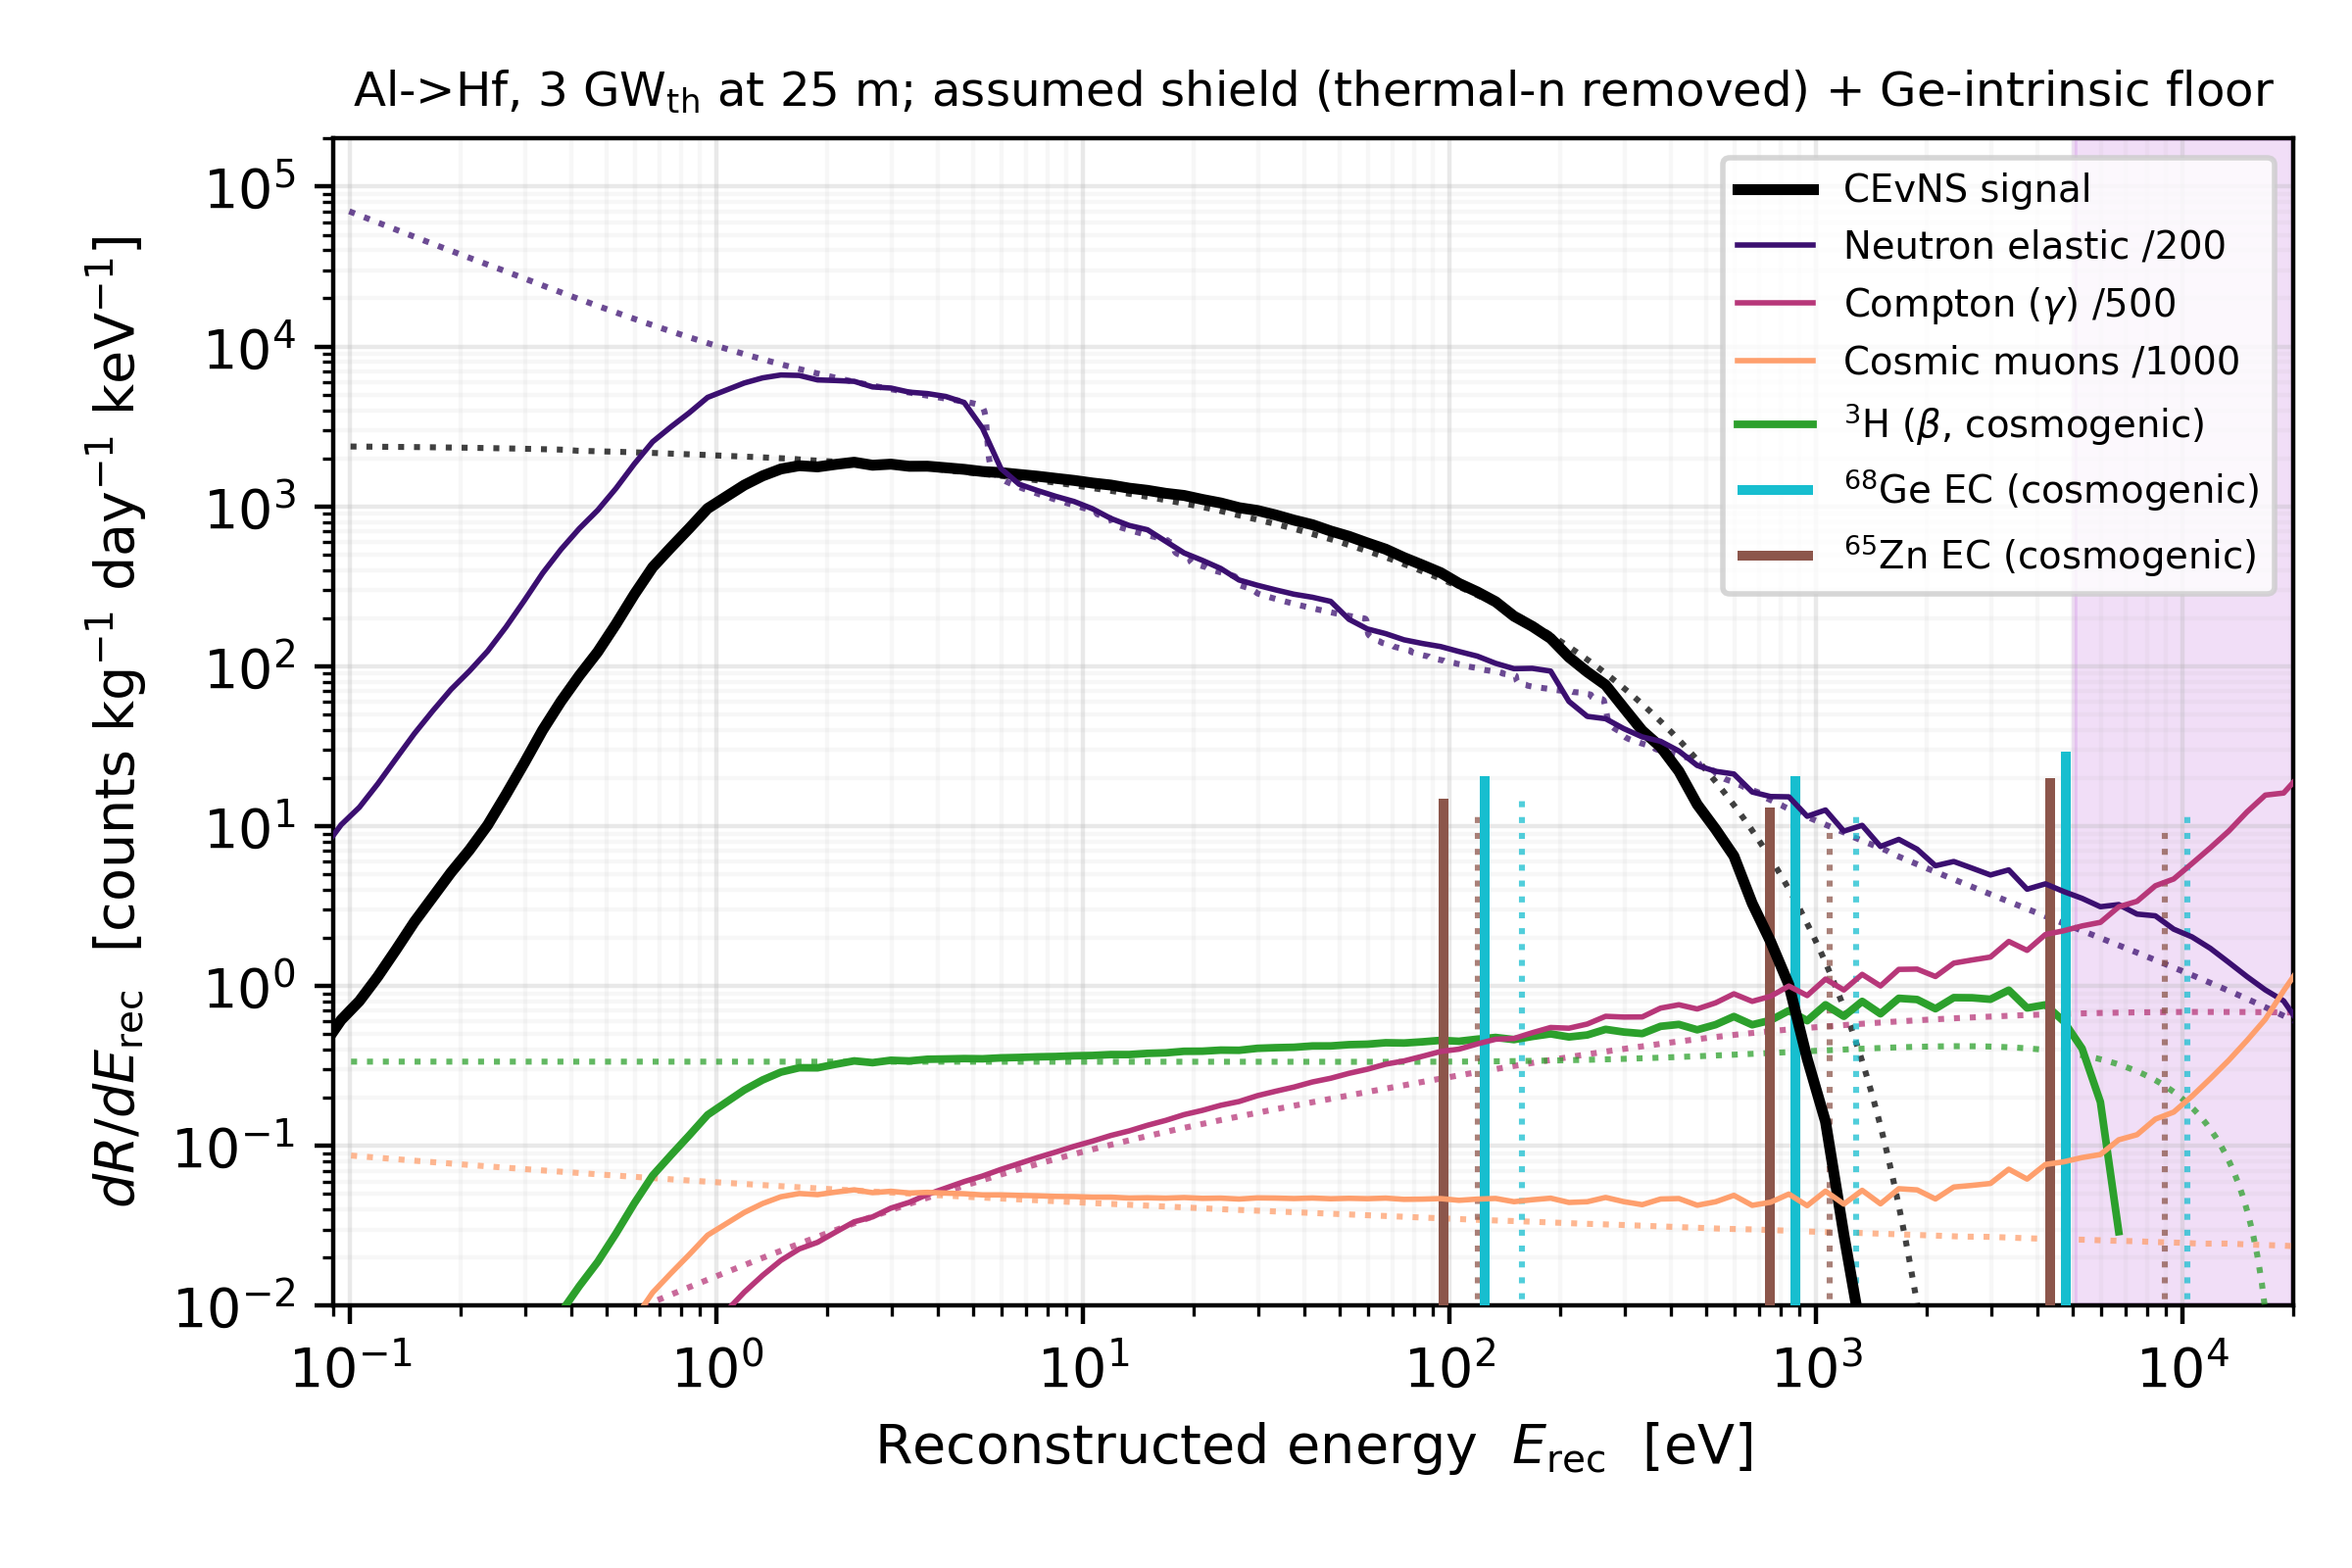
\includegraphics[width=0.72\textwidth]{figures/shielded_scenario_spectrum.png}
\caption{Central result: reconstructed-energy differential rate spectra $dR/dE_{\rm rec}$ (counts~kg$^{-1}$~day$^{-1}$~keV$^{-1}$) for the Al$\to$Hf design under non-paralyzable censoring, in the assumed-shield scenario (Ta$\to$Al is qualitatively identical). The reconstructed energy is calibrated to estimate the deposited energy. The reactor-CEvNS signal (black, thick) reconstructs to tens of eV. The ambient neutron-elastic recoils (purple) occupy the same band and, even after the assumed neutron suppression factor of $200$ shown, are the dominant background there; cosmic-muon deposits (orange, suppressed by the assumed factor $1000$ veto) span $\sim$1.5--197~MeV yet pile up at tens of keV---an instrumental artifact of the bandwidth ceiling, not a physical line; the environmental-gamma Compton continuum (magenta, suppressed by the assumed factor $500$) fills the region between. The Ge-intrinsic cosmogenic floor---$^{3}$H (green), $^{68}$Ge and $^{65}$Zn electron-capture lines (cyan and brown stems)---is drawn unsuppressed, as no external shield reaches it. Solid curves are the reconstructed (saturated, triggered) spectra; dotted curves are the corresponding linear-response, pre-saturation forms. Shaded purple marks the bandwidth-saturated region. The suppression factors are the assumed-shield modeling inputs of Sec.~\ref{sec:backgrounds}, quoted in the legend.}
\label{fig:spectra}
\end{figure*}
\begin{figure}
\centering
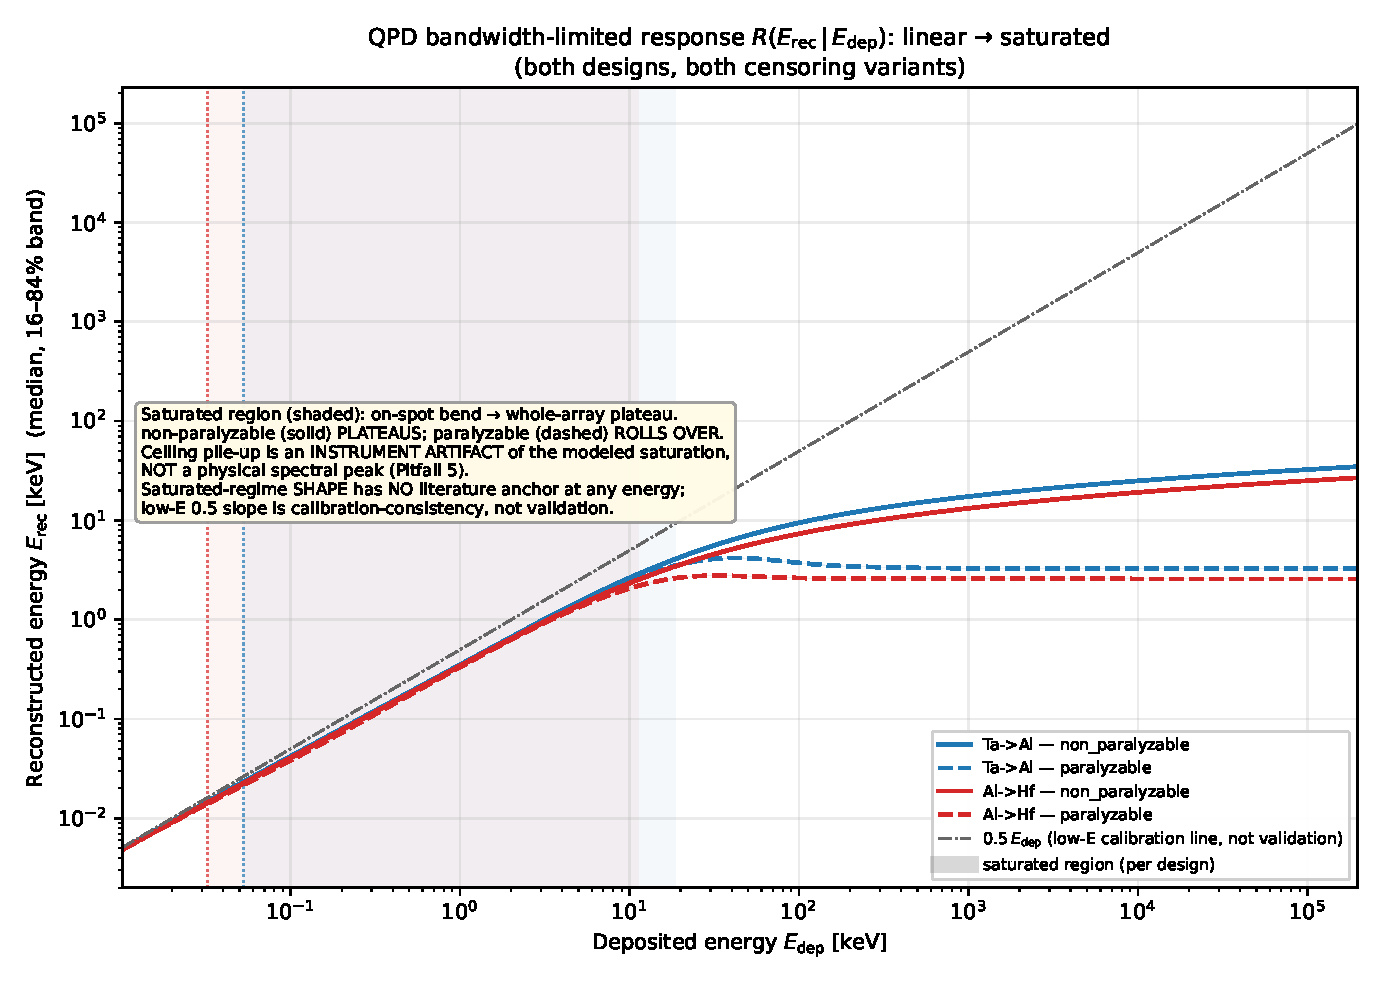
\includegraphics[width=\columnwidth]{figures/energy_response.pdf}
\caption{Monte-Carlo QPD response $R(E_{\rm rec}\,|\,E_{\rm dep})$ for both designs and both censoring variants, showing the linear $E_{\rm rec}\approx E_{\rm dep}$ regime (the reconstructed energy calibrated to estimate the deposit), the crossover onset, and the saturation plateau.}
\label{fig:response}
\end{figure}
\begin{figure}
\centering
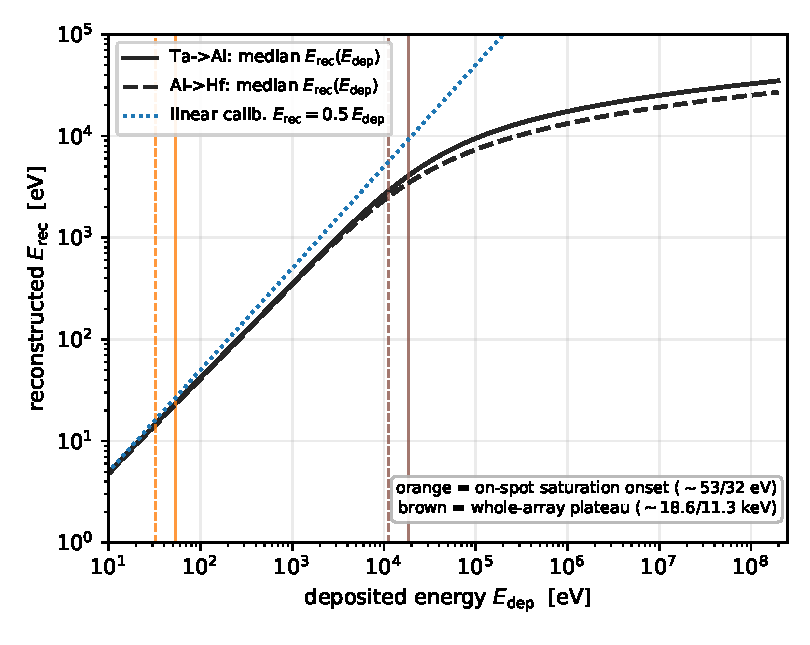
\includegraphics[width=\columnwidth]{figures/true_reconstructed_mapping.pdf}
\caption{True-to-reconstructed energy mapping: the median non-paralyzable response $E_{\rm rec}(E_{\rm dep})$ for both trapping designs (Ta$\to$Al solid, Al$\to$Hf dashed), with the on-spot saturation-onset (orange) and whole-array-plateau (brown) deposit scales and the linear-calibration reference $E_{\rm rec}=E_{\rm dep}$ (dotted). Below the onset the mapping is linear (the reconstructed energy estimates the deposit); above it the reconstructed energy rolls onto the bandwidth-limited saturation plateau. Nothing below 10~eV is displayed.}
\label{fig:mapping}
\end{figure}
\begin{figure}
\centering
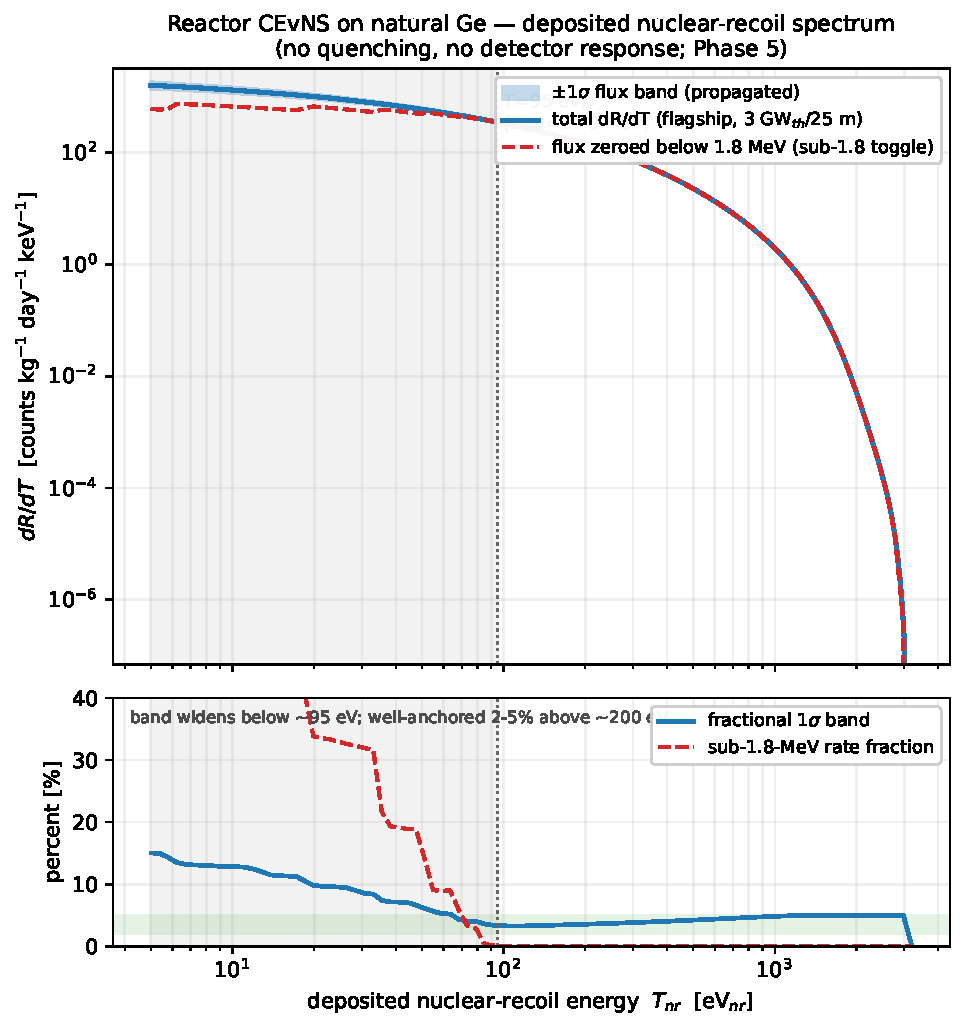
\includegraphics[width=\columnwidth]{figures/cevns_dRdT_deposited.pdf}
\caption{Deposited nuclear-recoil differential CEvNS rate $dR/dT$ on natural germanium at 3~GW$_{\rm th}$ and 25~m, with the split flux-uncertainty band and the Billard-benchmark reproduction.}
\label{fig:cevns}
\end{figure}

\begin{acknowledgments}
This research made use of Get Physics Done (GPD), developed by Physical Superintelligence PBC (PSI).
\end{acknowledgments}

\appendix
\section{Cross-section and form-factor conventions}
\label{sec:appendix-cevns}
This appendix collects the cross-section and form-factor detail deferred from Sec.~\ref{sec:cevns}: the full Freedman differential cross section with its normalization conventions, the closed-form total against which the differential is checked, the Lewin--Smith Helm form factor and its parameters, and the per-isotope natural-germanium table that enters the fold of Eq.~\eqref{eq:cevnsfold}.

\subsection{Freedman cross section and closed-form check}

For a neutrino of energy $E_\nu$ scattering coherently off isotope $i$ with recoil energy $T\equiv E_{\rm nr}$, we use the Freedman standard-model cross section~\cite{freedman1974,drukier1984}
\begin{equation}
\frac{d\sigma_i}{dT} = \frac{G_F^2 M_i}{4\pi}\, Q_{W,i}^2
\left(1 - \frac{M_i T}{2 E_\nu^2}\right) F_i^2(q)\,(\hbar c)^2 ,
\label{eq:app-dsigma}
\end{equation}
with the Fermi constant $G_F$, nuclear mass $M_i$, and weak charge $Q_{W,i}=N_i-(1-4\sin^2\theta_W)Z$ evaluated at $\sin^2\theta_W=0.2387$ (low-energy $\overline{\rm MS}$ value, not the $M_Z$ value $0.2312$) and $Z=32$. Two normalization choices are load-bearing and are the most common reactor-CEvNS errors: the $/4\pi$ prefactor (the $/8\pi$ form is a factor-of-two error), and the explicit conversion $(\hbar c)^2=3.894\times10^{-28}$~GeV$^2$cm$^2$ that restores the natural-unit cross section (evaluated with $G_F$ in GeV$^{-2}$, $M_i$ and $E_\nu$ in GeV) to cm$^2$. Because $1-4\sin^2\theta_W=0.0452$ the proton coupling nearly vanishes and $Q_{W,i}^2$ scales as $N_i^2$ to $\sim0.5\%$. The kinematic factor $(1-M_iT/2E_\nu^2)$ enforces the endpoint $T_{\max}^{(i)}(E_\nu)=2E_\nu^2/(M_i+2E_\nu)$, and each fold in Eq.~\eqref{eq:cevnsfold} runs above $E_\nu^{\min,(i)}(T)=\tfrac12\!\left(T+\sqrt{T^2+2M_iT}\right)\simeq\sqrt{M_iT/2}$.

Setting $F_i=1$ and integrating Eq.~\eqref{eq:app-dsigma} over $0\le T\le T_{\max}$ uses $\int_0^{T_{\max}}(1-M_iT/2E_\nu^2)\,dT=E_\nu^2/M_i$, giving the closed-form total
\begin{equation}
\sigma_{{\rm tot},i}(E_\nu) = \frac{G_F^2 Q_{W,i}^2 E_\nu^2}{4\pi}\,(\hbar c)^2 .
\label{eq:app-sigmatot}
\end{equation}
Our differential reproduces Eq.~\eqref{eq:app-sigmatot} to a relative $3\times10^{-9}$--$6\times10^{-8}$ across the five isotopes and $E_\nu\in\{2,4,8\}$~MeV, and yields $\sigma({}^{72}\mathrm{Ge},4~\mathrm{MeV})=1.0026\times10^{-40}$~cm$^2$, $0.26\%$ from the first-principles $1.0\times10^{-40}$~cm$^2$ anchor. Dimensionally $[G_F^2 M_i E_\nu^2]=\mathrm{GeV}^{-1}$, and $(\hbar c)^2$ carries the remaining $\mathrm{GeV}^2\mathrm{cm}^2$, so $d\sigma/dT$ is in cm$^2$/GeV with $Q_W^2$, the kinematic factor, and $F^2$ dimensionless.

\subsection{Lewin--Smith Helm form factor}

The nuclear form factor is the Lewin--Smith parametrization~\cite{lewinsmith1996} of the Helm ansatz~\cite{helm1956},
\begin{equation}
F(q) = \frac{3\, j_1(qR_0)}{qR_0}\,\exp\!\left(-\tfrac12 q^2 s^2\right),
\qquad
R_0^2 = c^2 + \tfrac{7}{3}\pi^2 a^2 - 5 s^2 ,
\label{eq:helm}
\end{equation}
with $j_1$ the first spherical Bessel function, diffraction radius $c=1.23\,A^{1/3}-0.60$~fm, surface diffuseness $a=0.52$~fm, and skin thickness $s=0.90$~fm; $F(0)=1$ by construction. The momentum transfer $q=\sqrt{2M_iT}$ is expressed in fm$^{-1}$ via $q[\mathrm{fm}^{-1}]=q[\mathrm{MeV}]/(\hbar c)$ with $\hbar c=197.327$~MeV\,fm, so that $qR_0$ and $qs$ are dimensionless (feeding $q$ in the wrong units produces a large spurious suppression). For germanium at reactor recoils the form factor is nearly unity: $F^2>0.998$ in the sub-$100$~eV region that carries most of the rate, falling to $F^2({}^{72}\mathrm{Ge})=0.9963$ at $T=200$~eV and to $0.9639$ only at the rare $\sim\!2$~keV endpoint reached by $E_\nu\sim8$--$10$~MeV neutrinos. These are consistent: the $>0.998$ figure is the dominant low-recoil regime and the $\sim\!0.96$ value is the high-recoil tail. The integrated deposited rate above $50$~eV is form-factor independent at the sub-percent level---turning $F$ off shifts it by $0.38\%$---so reactor CEvNS on Ge sits in the form-factor-insensitive regime and the exact skin parameters are not a systematic driver.

\subsection{Natural-germanium isotope table}

The fold retains each stable isotope's own weak charge, nuclear mass, kinematic endpoint, and number abundance rather than a lumped-$A$ approximation, which would smooth the five-step endpoint structure and bias the near-threshold and near-endpoint bins. Table~\ref{tab:ge-isotopes} lists the five isotopes, with $M_i=A_i\times931.494$~MeV and $T_{\max}^{(i)}$ at the $E_\nu=10$~MeV reactor endpoint; the per-isotope target density is $N_{T,i}=x_i\times8.29\times10^{24}$~kg$^{-1}$ ($\sum_i N_{T,i}=8.29\times10^{24}$~kg$^{-1}$). The five distinct endpoints ($2824$--$3066$~eV) produce the stepped superposition seen at the high-recoil edge of $dR/dT$.

\begin{table}[t]
\centering
\caption{The five stable natural-germanium isotopes ($Z=32$) entering the CEvNS fold of Eq.~\eqref{eq:cevnsfold}: neutron number $N_i$, number abundance $x_i$ (IUPAC/CIAAW representative values, $\sum_i x_i=1$), nuclear mass $M_i=A_i\times931.494$~MeV, and kinematic endpoint $T_{\max}^{(i)}$ at the $E_\nu=10$~MeV reactor endpoint.}
\label{tab:ge-isotopes}
\begin{ruledtabular}
\begin{tabular}{lcccc}
Isotope & $N_i$ & $x_i$ & $M_i$ (GeV) & $T_{\max}^{(i)}$ (eV) \\
\colrule
${}^{70}$Ge & 38 & 0.2057 & 65.13 & 3066 \\
${}^{72}$Ge & 40 & 0.2745 & 66.99 & 2981 \\
${}^{73}$Ge & 41 & 0.0775 & 67.93 & 2940 \\
${}^{74}$Ge & 42 & 0.3650 & 68.86 & 2901 \\
${}^{76}$Ge & 44 & 0.0773 & 70.72 & 2824 \\
\end{tabular}
\end{ruledtabular}
\end{table}

The ${}^{73}$Ge nuclear spin contributes a spin-dependent axial term that is $\sim\!1/N^2$ suppressed and negligible for the coherent rate; we state it but do not model it.

\section{Response-matrix Monte Carlo and convergence}
\label{sec:appendix-response}
This appendix supplies the microphysical detail deferred from Sec.~\ref{sec:response}: the tunneling-burst model that turns a per-sensor share into an event train, the single-constant calibration of the count-integral estimator, the Monte-Carlo construction and convergence of the response matrix $R(E_{\rm rec}\,|\,E_{\rm dep})$, and the parameter scan that turns the crossover into a band.

\emph{EMG tunneling-burst model.} On each sensor the trapped-quasiparticle population set by a share $E_s$ drives a two-exponential pulse [Ref.~\cite{ramanathan2026}, Eq.~4], $N_{\rm qp}(t)=\tau_{\rm qp}N_{\rm qp}\,g(t)$ with unit-area shape $g(t)=(e^{-t/\tau_{\rm qp}}-e^{-t/\tau_{\rm inj}})/(\tau_{\rm qp}-\tau_{\rm inj})$, so the instantaneous tunneling rate is $\Gamma_{\rm in}(t)=(K/V_{\rm tr})N_{\rm qp}(t)$. Here $\tau_{\rm qp}$ is the trapped-quasiparticle lifetime, $\tau_{\rm inj}$ the injection time, $K$ the tunneling-rate constant, and $V_{\rm tr}$ the trap volume. The tunneling events form a burst with exponentially-modified-Gaussian (EMG) arrival times, realized with the \texttt{QuasiparticleBurstModel} template of Ref.~\cite{ramanathan2026}; its EMG parameters $(\tau,\mu,\sigma)$ are fixed once per design so that the pdf peak reproduces $\max_t g(t)=p/\tau_{\rm qp}$ (recorded peak factors $p=0.25$ for Al, $0.13$ for Hf). The Poisson mean supplied to the template is the expected number of \emph{tunneling events},
\begin{equation}
n_{\rm ev}=\int_0^\infty \Gamma_{\rm in}(t)\,dt=\frac{K\,\tau_{\rm qp}}{V_{\rm tr}}\,N_{\rm qp},
\label{eq:eventcount}
\end{equation}
a dimensionless count that is \emph{not} the trapped population $N_{\rm qp}$: the two differ by the prefactor $K\tau_{\rm qp}/V_{\rm tr}\simeq0.03$ (Al) and $\simeq0.008$ (Hf). Feeding $N_{\rm qp}$ instead of $n_{\rm ev}$ would mis-scale the saturation onset by these factors, so Eq.~\eqref{eq:eventcount} is enforced everywhere the burst is realized.

\emph{Count-integral calibration.} Each realized event train is censored by the non-paralyzable dead-time model [Eq.~\eqref{eq:censor}] to a per-sensor observed count, and the array sum $N_{\rm obs}$ is mapped to energy by $E_{\rm rec}=C\,N_{\rm obs}$ [Eq.~\eqref{eq:erec}]. The constant $C$ (eV per event) is a \emph{single global} value per design, fixed once on a deeply unsaturated deposit ($E_{\rm dep}=0.01$~eV, no sensor near the ceiling) by requiring $dE_{\rm rec}/dE_{\rm dep}=1$, i.e.\ calibrating the reconstructed energy to estimate the deposited energy; this absorbs the physical yield fraction $\varepsilon$ into $C$, exactly as calibrating against a known line would. Because the unsaturated summed count is exactly proportional to $E_{\rm dep}$, one point fixes $C$; it is never retuned per bin. The recovery of $E_{\rm rec}\approx E_{\rm dep}$ at low energy is therefore a calibration-consistency check (verified to $<1\%$ for both designs), while the deep-saturation plateau is the genuinely predictive content: with censoring disabled the estimator returns exactly $E_{\rm dep}$ at all energies, so the plateau is the modeled bandwidth ceiling and not a numerical artifact.

\emph{Response-matrix Monte Carlo and convergence.} Each $E_{\rm dep}$ column of $R$ is built by histogramming $N_s=5000$ forward realizations of Eq.~\eqref{eq:erec}, on a grid of $584$ deposits sampled uniformly in $\log E_{\rm dep}$ from $10.14$~eV to $197$~MeV ($\simeq$80 bins per decade), the shared grid on which Sec.~\ref{sec:results} folds the deposit spectra. The $\sim\pi r^2$ on-spot sensors are realized individually; the $\sim$10,287 identical off-spot sensors are drawn as one aggregate multinomial ensemble per realization rather than looped. Columns normalize to unity to $10^{-12}$. The per-cell relative Monte-Carlo error is Poisson,
\begin{equation}
\epsilon_{jk}=\frac{1}{\sqrt{N_{jk}}}=\frac{1}{\sqrt{N_s\,R_{jk}}},
\label{eq:mc-converge}
\end{equation}
with $N_{jk}$ the count in cell $(j,k)$; the well-populated (peak) cell reaches $\epsilon\lesssim1.8\%$ at $N_s=5000$ with clean $1/\sqrt{N_s}$ scaling, and every column is reproducible across processes via deterministic \texttt{crc32} sub-seeding. One honesty split is required: where the event count is feasible ($n_{\rm ev}\le2000$) the burst is realized with the full EMG template, but in deep saturation the train would carry $\mathcal{O}(10^8)$ events and is infeasible to materialize, so there the registered count is drawn Poisson about the analytic censored mean. In that regime the relative spread of the summed $E_{\rm rec}$ is $\sim10^{-3}$---the column is effectively a delta---so the approximation is immaterial to $R$; the per-class mean is pinned to the validated analytic estimator in both branches, leaving no kink at the split.

\emph{Crossover-band scan.} The on-spot sensor saturates first, at the per-sensor onset share $E_{\rm onset}$ ($\simeq1.27$~eV for Ta$\to$Al, $\simeq0.77$~eV for Al$\to$Hf); inverting the sharing partition gives the crossover deposit energy $E_{\rm dep}^{\rm cross}$ of Eq.~\eqref{eq:crossover}. Scanning the low-confidence sharing parameters over $f_{\rm prompt}\in[0.1,0.5]$ and $r\in[1,5]$ spreads this from $\sim$8~eV to $\sim$0.93~keV (Ta$\to$Al) and $\sim$4.8~eV to $\sim$0.57~keV (Al$\to$Hf) about the default $\sim$52.9/32.1~eV, the $f_{\rm prompt}$-dominated band quoted in Sec.~\ref{sec:response}. Two limiting anchors bound it: the equal-split limit $f_{\rm prompt}\to0$, where every sensor shares equally and all saturate together, and the whole-array plateau at the default $f_{\rm prompt}$, where even the diffuse share reaches onset,
\begin{align}
E_{\rm dep}^{\rm equal\text{-}split} &= E_{\rm onset}\,N_{\rm sens}, \nonumber\\
E_{\rm dep}^{\rm plateau} &= \frac{E_{\rm onset}\,N_{\rm sens}}{1-f_{\rm prompt}},
\label{eq:onset-band}
\end{align}
with $N_{\rm sens}\simeq10{,}300$. These evaluate to $\sim$13.1~keV (equal-split) and $\sim$18.6~keV (plateau) for Ta$\to$Al, and $\sim$7.9~keV and $\sim$11.3~keV for Al$\to$Hf. The Al$\to$Hf design, with the lower per-sensor onset, saturates before Ta$\to$Al at every point of the scan.

\bibliography{references}

\begin{center}
{\footnotesize\textit{Generated with Get Physics Done}}
\end{center}

\end{document}